%%%%%%%%%%%%%%%%%%%%%%%%%%%%%%%%%%%%%%%%%% University Assignment Title Page 
% LaTeX Template
% Version 1.0 (27/12/12)
%
% This template has been downloaded from:
% http://www.LaTeXTemplates.com
%
% Original author:
% WikiBooks (http://en.wikibooks.org/wiki/LaTeX/Title_Creation)
%
% License:
% CC BY-NC-SA 3.0 (http://creativecommons.org/licenses/by-nc-sa/3.0/)
% 
% Instructions for using this template:
% This title page is capable of being compiled as is. This is not useful for 
% including it in another document. To do this, you have two options: 
%
% 1) Copy/paste everything between \begin{document} and \end{document} 
% starting at \begin{titlepage} and paste this into another LaTeX file where you 
% want your title page.
% OR
% 2) Remove everything outside the \begin{titlepage} and \end{titlepage} and 
% move this file to the same directory as the LaTeX file you wish to add it to. 
% Then add \input{./title_page_1.tex} to your LaTeX file where you want your
% title page.
%
%%%%%%%%%%%%%%%%%%%%%%%%%%%%%%%%%%%%%%%%%
%\title{Title page with logo}
%----------------------------------------------------------------------------------------
%	PACKAGES AND OTHER DOCUMENT CONFIGURATIONS
%----------------------------------------------------------------------------------------

\documentclass[12pt]{article}
\usepackage[utf8]{inputenc} % remove x to make it compatible to biblography
\usepackage[T1]{fontenc} % added instead of utf8x
\usepackage{textcomp} % added instead of utf8x

\usepackage{amsfonts,amssymb,amsmath,amsthm}
\usepackage{graphicx}
\usepackage{subcaption}
\usepackage[colorinlistoftodos]{todonotes}
\usepackage{caption}
\usepackage{float}
\usepackage{verbatim}
\usepackage{ragged2e}
\usepackage[hyphens]{url} % quick and dirty fix to the overflowing url problem
\usepackage{hyperref}
\usepackage{csquotes}
\usepackage{booktabs}
\usepackage{siunitx}
\usepackage{makecell}

\usepackage[backend=biber, style=authoryear, autocite=inline]{biblatex}
\addbibresource{sources.bib}

\setlength\parindent{0pt}
\setlength\bibitemsep{1.5\itemsep}

\renewcommand{\arraystretch}{2.2}

\justifying
\renewcommand*\contentsname{Content}
\begin{document}

\begin{titlepage}

\newcommand{\HRule}{\rule{\linewidth}{0.5mm}} % Defines a new command for the horizontal lines, change thickness here

\center % Center everything on the page
 
%----------------------------------------------------------------------------------------
%	HEADING SECTIONS
%----------------------------------------------------------------------------------------

\textsc{\LARGE Data Science Semester Project}\\[1.5cm] % Name of your university/college
\textsc{\large{Author: }Julien Heitmann}\\[0.5cm] % Major heading such as course name

%----------------------------------------------------------------------------------------
%	TITLE SECTION
%----------------------------------------------------------------------------------------

% Neural network pruning and weight geometry

\HRule \\[0.6cm]
{ \huge \bfseries Sources of Redundancy in Neural Networks}\\[0.5cm] % Title of your document
\HRule \\[1.5cm]
 
%----------------------------------------------------------------------------------------
%	AUTHOR SECTION
%----------------------------------------------------------------------------------------


% If you don't want a supervisor, uncomment the two lines below and remove the section above
%\Large \emph{Author:}\\
%John \textsc{Smith}\\[3cm] % Your name

%----------------------------------------------------------------------------------------
%	DATE SECTION
%----------------------------------------------------------------------------------------
\begin{figure}[!h] 
        \centering 
\includegraphics[width=0.6\columnwidth]{images/EPFL_Logo_Digital_RGB_PROD.jpg}
\end{figure}

\vfill % Fill the rest of the page with whitespace
\end{titlepage}
\tableofcontents
\newpage
\justify

\setlength\parindent{0pt}

\section{Introduction}
One of the suprising results of training deep neural networks with many more parameters than training samples is that one can achieve zero-training loss but still get good generalisation ~~\autocite{neyshabur2018towards}. While statistical learning theory suggests that such heavily over-parametrised networks generalise poorly without further regularisation, experiments show that in most cases, increasing the number of parameters does not worsen the capability to generalise. In fact, it often happens that, when training two models with $N1$ and $N2$ neurons respectively, $N1 > N2$, training will converge to zero-training loss in both cases, but the larger model will generalise better. This paradox is one of the big unresolved questions of deep learning, and understanding the phenomena behind it would deliver a lot of insights about why neural networks work so well. The question arises why the network doesn't exploit its full expressive power to overfit the training dataset. Modern network architectures, which can have up to 100x more trainable parameters than training samples ~\autocite{zagoruyko2016wide}, most certainly are capable of learning the entire dataset, independently of the labels. It has been shown that zero training loss can even be achieved when the training labels are randomly shuffled ~\autocite{zhang2016understanding}, thus preventing the learning of underlying features of the data that are sufficient to solve the classification task at hand. \\

Surely one must look at the interplay between the dataset properties, the network architecture and the optimization algorithm, but the latter in particular seems to play a crucial role, as it somehow consistently favors solutions in the optimization landscape that generalize, over solutions that overfit the data and in some cases do not learn a representation of the data. Is it a property of the optimization algorithm, does stochastic gradient descent optimization lead to sparse solutions? If yes, how do these sparse solutions look like? Do trained neural networks rely on single components (nodes or filters), even with a growing number of parameters? Or does each of the components contribute equally to the estimated function, thus reducing the contribution when there are more parameters? \\

An interesting way to measure the importance of a trained network's individual components is pruning. When single components are removed from a network's architecture, i. e. they do not contribute anymore to the output of the network, the difference in validation accuracy can be measured, which is a good indicator of the network's performance. Pruning can therefore be used as a means to get a better understanding of what is happening in a trained network, to identify important parts and not so important ones. But pruning can also be seen as an end, if done properly it might yield smaller architectures, which result in computation speed-ups and smaller memory footprints at evaluation. Assuming that over-parameterization is necessary to achieve good performance and generalization, and that some components of an over-parameterized network are obsolete after training or can be removed without a negative impact on validation accuracy if the network is retrained, then pruning might even be necessary to get efficient architectures that scale. \\

This project aims to explore different hypotheses about neural network training dynamics, with a particular focus on pruning. The goal is to identify both similarities and differences in the theories, and provide evidence in favor or against them in a series of experiments. Moreover, some visualization tools will be introduced that will help getting a better intuition for the complex process that is neural network training.

\subsection{Formal background}

Formally define frame potential, generalization error, network architecture, optimization algorithms. 

\section{Related work}
\label{section:prior}
% improve this part, deconstruct classification subspace
If good generalization can be achieved by an overparameterized network, there must be some mechanism that prevents the model to overfit the dataset, and learn for instance features that would be considered as noise when it comes to the classification task, because they do not provide any information about a sample's affiliation to a certain class. With an increasing number of parameters, more complex decision boundaries can be represented, so in order to generalize, the solutions obtained by the optimization algorithm of choice must be "simple" in a way, which is yet to be defined. While it is curious that large neural networks do not overfit the dataset, even in the presence of massive label noise ~\autocite{rolnick2017deep}, it is even more surprising that increasing the number of parameters can decrease the generalization gap ~\autocite{neyshabur2018towards}. In other words, given a classification task and a certain model architecture with a fixed number of layers but adjustable layer widths, a certain degree of layer-wise over-parameterization might be both sufficient and necessary to achieve good performance after training. 

\subsection{Self-regularization of over-parameterized models}
The inability of statistical learning to explain and predict the properties of neural networks is not a new phenomenon. In particular, when it comes to measuring complexity, traditional measures such as the VC dimension or the number of parameters fail to explain why increasing the number of parameters of a model does not necessarily increase the generalization gap. More recently new measures have been introduced that aim to take into account the self-regularizing effect observed during the training of large models. For instance, \cite{neyshabur2018towards} 
 measure a network's capacity by looking at the Frobenius norm of the difference of the hidden layer weights with the initialization, and empirically show that this measure decreases with increasing network size. This suggests that the bigger the network, the smaller the work the optimization algorithms needs to do, since the hidden layer weights are closer to their initialization. \\

Furthermore one should keep in mind, when examining a model's capacity, that the notion of overparameterization itself is very vague, as it is intractable to measure a classification problem's complexity, and therefore determine the appropriate number of parameters. Experiments involving teacher-student models avoid this problem and are thus easier to analyze. The teacher is a model with a specific architecture and fixed weights, that given a random input produces an output. This generative process is repeated multiple times, and the input-output pairs are given to a student model as training data. The student is a model with a similar architecture, but a larger number of hidden units, and the goal for the student is to learn the teacher's model. Because the student can express much more complex functions than the teacher function it has to learn, it is said to be over-parameterized. \cite{goldt2019dynamics} found evidence that, with a teacher-student setup, upon over-parameterization Stochastic Gradient Descent finds solutions which amount to performing an effective model averaging, thus improving robustness and avoiding overfitting. \\

This property seems to extend to more practical problems than the artificial teacher-student setup, there has been empirical evidence that supports that repeated units emerge when increasing a network's width, as a way to adjust the capacity of the model ~\autocite{casper2019removable}. Those repeated units have highly correlated outputs, implying that similar activation regions were learned. Additionally, removable units appear, which can be dropped out of the network without significantly hurting the validation accuracy. This kind of self-regularization enforces capacity constraints, as the function modeled by a network with either of these units could me modeled by a simpler one. \\
 
The emergence of repeated or removable units during the training process of large models indicates that the self-regularizing mechanism that allow overparameterized networks to generalize after training opperate at least partly at the level of individual units. There has been work that makes use of recent advances in Random Matrix Theory (RMT) to describe the different phases of that implicit self-regularization of the weight matrices ~\autocite{martin2018implicit}. More specifically, the Empirical Spectral Density (ESD) of the correlation matrix $\mathbf{X} = \mathbf{W}\mathbf{W}^T$ associated with the layer weight matrix $\mathbf{W}$ is analysed over the course of training. RMT is used to identify different phases of training using models to describe the shape of each ESD. In each phase the layer weight matrix $\mathbf{W}$ is modeled as "noise plus signal", where the noise is modeled by a random matrix $\mathbf{W}^{rand}$, which entries are drawn from a normal distribution, and the signal is a correction $\Delta^{sig}$, $\mathbf{W} \simeq \mathbf{W}^{rand} + \Delta^{sig}$. The empirically verified models suggest that during training, $\mathbf{W}^{rand}$ decreases, and $\Delta^{sig}$, a low-rank matrix, increases in magnitude. The hypothesis that, when training an overparameterized network, only a low-rank subspace of the weight matrices is relevant for the learning target has also been put forward by \cite{nagarajan2019uniform}. To support their claims they analyze the singular value distribution of the update matrix $\mathbf{W} - \mathbf{Z}$, which is the difference between the final weight matrix $\mathbf{W}$ and the weight matrix at initialization $\mathbf{Z}$. They show that the validation accuracy is able to endure the heavy pruning process of projecting the update matrix onto its top 16 left-singular vectors (out of 1024), and conclude that all but a few top singular directions can be considered as noise. They also notice that the spectral norm of the matrix (the residuals) that is removed when projecting onto the top singular vectors can have quite a high spectral norm. These results highlight the fact that low-complexity solutions are found when training networks that have a high representational power and, that even in the presence of noise introduced by SGD, the low-complexity component of the solution dominates the output of the network. \\


\subsection{Advantageous properties of over-parameterized models}
After looking at capacity constraining mechanisms in overparameterized neural networks, there is yet another, more intriguing question that needs to be answered: why can overparameterized neural networks achieve better generalization than smaller networks, even in cases such as a teacher-student setup where the smaller network is a student whose architecture matches that of the teacher ~\autocite{tian2019luck}? In an attempt to provide an answer to that question, a closer look will be taken at two theories that motivated some of the first steps of the project. The first one, more formaly known as the "Lottery ticket hypothesis" ~\autocite{frankle2018lottery}, emphasises the importance of weight initialisation, which leads to the formation of subnetworks that can be trained efficiently. The second one states that overparametrisation works well because of better feature exploration and weight clustering ~\autocite{brutzkus2019larger}.

%We can ask specific questions when reasoning about sparsity: within an overparametrised network, is it just a subnetwork that is trained, particularly receptive to training and with an inductive bias that makes it "trainable"? Or is there a collapse of the weight vectors around just a few directions, relevant to the classification task at hand? These questions correspond to different explanations of the underlying mechanisms of neural network training, and have been studied in the past.%

\subsubsection*{The Lottery Ticket Hypothesis}
Contemporary experience suggests that overparameterized networks are easier to train, and achieve better generalisation. But such networks can be pruned, which sometimes heavily reduces the parameter-count ~\autocite{han2015learning}. One might ask why we do not train instead architectures discovered by pruning. It is commonly believed that these pruned networks are more difficult to train from scratch, and reach lower accuracy than the fine-tuned pruned networks ~\autocite{li2016pruning}. The "Lottery ticket hypothesis" ~\autocite{frankle2018lottery} is a theory that provides an explanation as to why over-parameterized networks might perform better, and has gained a lot of popularity recently. It states the following: \\

\textit{A randomly-initialized, dense neural network contains a sub-network that is initialized such that - when trained in isolation - it can match the test accuracy of the original network after training for at most the same number of iterations.} \\

According to the authors, at initialization, some weights that form a sub-network "win the lottery", because the combination of their initial value and the way they are aranged in that particular sub-network makes them particularly "trainable" by the chosen optimization algorithm, compared to other weights that are not in the sub-network. Those weights form what is called a "winning ticket", and the paper provides a way to identify the winning ticket after multiple iterations of pruning, based on the weight magnitudes, and retraining, to compensate for the loss in accuracy caused by pruning. One of the important results of the paper is that when the weights of the winning ticket, which can be seen as a mask applied to the weights of the network, are reset to their initial value (all other weights set to zero), then the newly obtained network reaches similar if not better accuracy than the original network, up to a certain degree of pruning (up to 96\%). Surprisingly, this result does not hold when the weights of the winning ticket are re-sampled, meaning that both the pruned architecture and the values of the unpruned weights are of importance. When randomly re-sampled, the winning tickets learn slower and reach lower accuracy than the re-initialized one. \\

Note that, as individual weights are pruned to identify the winning ticket, the theory makes use of unstructured pruning, and a winning ticket obtained by this procedure would have to rely on speciliased libraries and hardware to exploit benefits of the weight matrix sparsity. According to \cite{liu2018rethinking}, the results do not hold when using structured pruning, and might even be misleading in the case of unstructured pruning. The authors of the paper claim that the optimization algorithm (ADAM) and the small initial learning rate of the original paper lead to inferior accuracy when the winning ticket is randomly initialized, but this can be remedied using SGD and a higher learning rate. Moreover, as claimed in the original paper, the procedure to identify a winning ticket fails for deeper networks. Nonetheless, according to Frankle and Carbin, even if in some cases, up to a certain level of sparsity, highly overparameterized networks can be pruned, reinitialized and retrained successfully, beyond a certain point, when the network is extremely pruned, less severely overparameterized networks only maintain a good validation accuracy if they are well-initialised. Also, winning tickets have been found for deeper networks ~\autocite{frankle2019lottery} when, instead of resetting the weights of the winning ticket to their initial values, they are rewinded to their former values at iteration $k$, where $k$ is much smaller than the total number of training iterations. Finally, winning tickets generate so much interest because they might reveal a lot about how to better initialise neural networks, but also help better understand the bias of modern optimization algorithms towards sparse solutions. Surprisingly, it has been shown that, within the natural images domain, winning ticket initialisations generalise across a variety of datasets, often achieving performance close to that of winning tickets generated on the same dataset ~\autocite{morcos2019one}. This suggests that winning tickets somehow have an inductive bias generic to neural networks, which generalizes to multiple configurations. 

\subsubsection*{Alignment of weight vectors during training}
\cite{brutzkus2019larger} define a simple 3-layer neural network for a binary classification task they call the XORD problem (XOR Detection). Its input is a vector with $2d$ entries, which take values in $\{-1, 1\}$, and the vector can be written as a sequence of $d$ pairs. The goal is to determine whether any of the pairs has twice the same value ($1$ or $-1$). For this purpose a neural network is trained, with a convolutional, a max-pool and a fully connected layer. Only the weights of the convolutional layer, which are vectors in $\mathbb{R}^2$, are trainable. The authors prove that increasing the size of the convolutional layer results in better feature exploration, and that after convergence the weight vectors associated to the learned convolutions cluster around just a few directions. Furthermore, they show that when the size of the convolutional layer is small (just a few trainable weights), the network can achieve zero-training error on specific datasets, but not generalize well, because it is missing some patterns. This is less likely to happen with a larger convolutional layer because of better exploration of the feature space. According to the authors, this might explain why over-parameterized neural networks don't overfit the training dataset and in some cases even generalize better than smaller networks. The former can be explained by weight clustering, which reduces the effective capacity of the network, and the latter by better exploration of the input space. Hence the observed generalization properties of over-parameterized networks do not contradict the findings of statistical learning, since training with gradient descent will facilitate the formation of clusters, thus reducing the network's expressive power. Empirically, the paper looks at a 3-layer neural network with a large convolutional layer, trained on MNIST. More specifically, after training, the vectors associated to the convolutional filters are clustered using K-Means with four clusters. The distribution of angles with respect to the closest cluster center is compared to that of clustered untrained vectors (at initialization). The findings are in accordance with the XORD theory, as trained vectors tend to be much closer to the center of the cluster they are part of.\\

Coming back to the second question: XOR-problem, sparse subspace spanned by trained vectors. Question arises: will optimization algorithms such as SGD enforce this alignment, therefore preventing overfitting? Interplay between vector alignment and "trainable" vectors. Goal is to explore and go beyond, understanding this mechanism will help us design better optimization algorithms, pruning methods, architectures, initialization methods, etc. Collapse at last layer?


\subsubsection*{Additional work}
Better exploration, luck and overlap, alignment of noise subspace.


\subsection{Leveraging model simplicity: Compression and Pruning}
Structured vs unstructured pruning, surprisingly leads to better generalization, pruning as a noise signal. Speed-up, memory foot-print. Need over-parameterized network for better exploration of hidden layer space (give examples), once the model converges / during training, remove useless components. Surprising results: prune components with highest magnitude, can lead to better test accuracy after re-training the pruned network.

\section{Results}

This project focuses on classification tasks on natural images datasets, solved by neural networks. It takes a weight-vector perspective when reasoning about the sources of redundancy and the effects of pruning. This means that only structured pruning will be performed, at the level of neurons or filters. Those will also be the main entities studied when trying to understand the properties of neural network optimization. Why not look at unstructured pruning / individual weights? \\

The fact that the lottery ticket hypothesis might not really apply at the level of nodes / filters ~\autocite{liu2018rethinking} could be due to multiple reasons:
\begin{itemize}
\item It is more difficult to identify winning tickets at the level of nodes or filters, i. e. iterative pruning based on the $\ell_2$-norm fails to identify elements that are part of the winning ticket
\item Structured pruning is to restrictive. Unstructured pruning can yield very complicated architectures that have at least one weight in every node or filter, even at high pruning ratios. This does not apply to structured pruning. 
\item Structured pruning is only efficient at low pruning rates, where the pruned architecture might be able to reach the same training loss when randomly initialized. Thus pruning can be done at the beginning, and there is no need to identify a winning ticket.
\end{itemize}

It would be interesting, from a theoretical point of view, to find out if, similarly to the well-initialized weights in the standard setting of the lottery ticket hypothesis, "trainable" nodes or filters exist. The hypothesis doesn't directly support this as, at a given layer, every node or filter should have the same expected number of weights which are in the winning ticket. But does that imply that, on average, at a given layer all nodes or filters are equally important and trained? In other words, are weights that are part of a winning ticket uniformly distributed across the nodes or filters of a layer, or do they concentrate on just a few of them?

Nonetheless, larger networks might still generalize better, and when we do not know how complex a classification task is or how big of a network we should use, then training an over-parameterized network can be interesting, especially if we are able to quickly identify "trainable" nodes or filters, so that other parameters can be pruned and training made faster. 

% simple architecture = only convolutional / fully connected layers
Assuming that the lottery ticket hypothesis is true, all nodes or filters of a layer in a neural network have the same probability of being part of the "trainable" subnetwork at initialization, that is having some weights that are in the winning ticket. Also, at every layer, all nodes or filters have the same expected number of weights in the winning ticket. 

Marginal distribution? Given that the node contains at least one weight that is part of the winning ticket, how does that affect the probability of other weights in the same node or filter of being part of the winning ticket?

\subsubsection*{Models}

\textbf{Add accuracy after convergence.}

\begin{figure}[H]
\centering
\scalebox{.65}
{\begin{tabular}{SSSSS} \toprule
    \textit{Network} & {LeNet} & {Conv-2} & {Conv-6} & {VGG19} \\ \midrule
    \textit{Convolutions} & {} & {64, 64, pool} & {\makecell{64, 64, pool \\ 128, 128, pool \\ 256, 256, pool}} & {\makecell{2x64 pool 2x128 pool \\ 4x256 pool 4x512 pool \\ 4x512 pool}} \\
    \textit{FC layers}  & {300, 100, 10} & {256, 256, 10} & {256, 256, 10} & {\makecell{avg-pool \\ 512, 512, 10}} \\
    \textit{All/Conv Weights}  & {266K} & {4.3M / 38K} & {1.7M / 1.1M} & {20.0M} \\
    \textit{Iterations/Batch}  & {50K / 64} & {20K / 64} & {40K / 60} & {112K / 64} \\
    \textit{Optimizer}  & {SGD 3e-3 Momentum 0.9} & {Adam 2e-4} & {Adam 3e-4} & {SGD 0.1-0.01-0.001 Momentum 0.9} \\ \bottomrule
\end{tabular}}
\caption{Architectures tested in this project. Convolutions are 3x3. Lenet is from \cite{lecun1998gradient}. Conv-2/4/6 are variants of VGG ~\autocite{simonyan2014very}. Initializations are Gaussian Glorot ~\autocite{glorot2010understanding}.}
\end{figure}

\subsection{Comparison of pruning criteria}

\subsubsection*{Starting point}
As we have seen, most modern pruning methods evaluate a component's importance based on its magnitude or $\ell_2$-norm (\textbf{CITE}). Even though this criterion delivers satisfying results, there isn't much theory to back it up, except for the greater contribution to the next layer's input or the final output, when averaged over all possible inputs. But this is not necessarily true for the input space, \cite{nagarajan2019uniform} show that the spectral norm of the weight matrices can be significantly reduced after training without affecting the validation accuracy too much. This so-called "noisy component" that is removed seems to have a bad alignment with the data and hence doesn't interfere too much with the parts that are more relevant to the output. Based on the findings of \cite{brutzkus2019larger}, we would like to investigate a new criterion to measure a weight vector's saliency that, instead of looking at magnitude, measures the "closeness" or "similarity" to other weight vectors. The idea that motivates this criterion is that, if indeed weight vectors get clustered during the training process, there might be some outliers that don't fall into any cluster and could be removed because they align poorly with the input data. \\

We would like to see if a pruning criterion that doesn't take magnitude into account can deliver satisfying results, so before working with a weight matrix $\mathbf{W}$, we normalize its rows and obtain $\hat{\mathbf{W}}$. To measure how "clustered" the weight vectors are at a given time in training, we use a metric called the \textit{frame potential} (FP), which is defined as follows for a normalized matrix $\hat{\mathbf{W}}$:

\begin{align*}
\text{FP}(\hat{\mathbf{W}}) = \sum\limits_{i,j} |\langle \hat{\mathbf{w}}_i, \hat{\mathbf{w}}_j \rangle|^2,
\end{align*}

where $\mathbf{w}_i$ are the normalized rows of $\hat{\mathbf{W}}$. Note that if we define the correlation matrix $\mathbf{X} =  \hat{\mathbf{W}}\hat{\mathbf{W}}^T$, then this can be rewritten as

\begin{align*}
\text{FP}(\hat{\mathbf{W}}) = \|\mathbf{X}\|_F^2 = \text{tr}(\mathbf{X}^T\mathbf{X}).
\end{align*}

\subsubsection*{Problem setup}
Consider a dense feed-forward neural network $f(x; \theta)$ with initial parameters $\theta = \theta_0 \sim \mathcal{D}_{\theta}$, corresponding to the weights of one input layer, $N$ hidden layers, and one output layer. When optimizing with Stochastic Gradient Descent (SGD) on a training set, $f$ reaches minimum validation loss $l$ at iteration $j$ with test accuracy $a$. The network has arrived at parameters $\theta_j$. Let $\mathbf{W}^L \in \mathbb{R}^{m \times n}$ be the weight matrix associated to the $L^{\text{th}}$ layer (input, hidden or output), at iteration $j$. Out of the $m$ units, we would like to remove $p < m$ of them such that, given the newly obtained test accuracy $a_p$ when dropping these units, the difference in accuracy $\Delta = a - a_p$ is minimized. Due to the combinatorial nature of the problem, we focus on greedy methods that iteratively remove units based on a certain criterion.  \\

\textit{Magnitude pruning}: Sort the weight vectors by their norm $\|\mathbf{w}_i\|, 1 \leq i \leq m$. Remove the weight vector with the smallest norm. Repeat the procedure $p$ times, updating the weight matrix accordingly. \\

\textit{Frame-potential pruning}: Sort the weight vectors by their contribution to the frame-potential, which for a weight vector $\mathbf{w}_i, 1 \leq i \leq m$, is $\sum\limits_{j=1}^m | \langle \hat{\mathbf{w}}_i, \hat{\mathbf{w}}_j \rangle |^2$, where $\hat{\mathbf{w}}_i, \hat{\mathbf{w}}_j$ are the normalized vectors. Remove the weight vector with the smallest contribution to the frame-potential. Repeat the procedure $p$ times, updating the weight matrix accordingly. \\

For the sake of comparison, we might want to remove $p < m$ units such that the difference in accuracy $\Delta = a - a_p$ is maximized, to study how much harm can be done to the trained network. Again, using magnitude or contribution to frame-potential as a metric to measure a unit's saliency, we can adapt \textit{Magnitude pruning} and \textit{Frame-potential pruning} such that the weight vector with the highest norm or the highest contribution to the frame-potential is removed, and repeat this procedure multiple times. \\

The effects of pruning without retraining were only studied for the smaller models LeNet and Conv-2. Random pruning, which removes individual units at random, has been added as a baseline. Other pruning metrics, that were not discussed in this report, have also been tested and should be disregarded.
The results are summarized in figures \ref{fig:lenet-fc1} and \ref{fig:conv2-fc1}.

\subsubsection*{Observations}
\textit{Magnitude pruning} performs better than \textit{Frame-potential pruning}, for both fully connected and convolutional layers (plots for convolutional layers not shown, they tell a similar story). Nonetheless, pruning strategies that maximize or minimize frame-potential of the pruned matrix show that angle with respect to other weight vectors is correlated with a unit's importance, which is measured through the observed difference in test accuracy. \texttt{max\_fp\_pruning} performs better than random pruning (much better in some cases as fig. \ref{fig:conv2-fc1} shows), and \texttt{min\_fp\_pruning} can significantly damage a network. This leads us to the next section, at this point it seemed necessary to further investigate the relationship between angle and magnitude of a unit, and a visualization that encodes both angle and magnitude allows us to better understand the dynamics between the two.

\begin{figure}[H]
\centering
\begin{subfigure}[b]{\textwidth}
   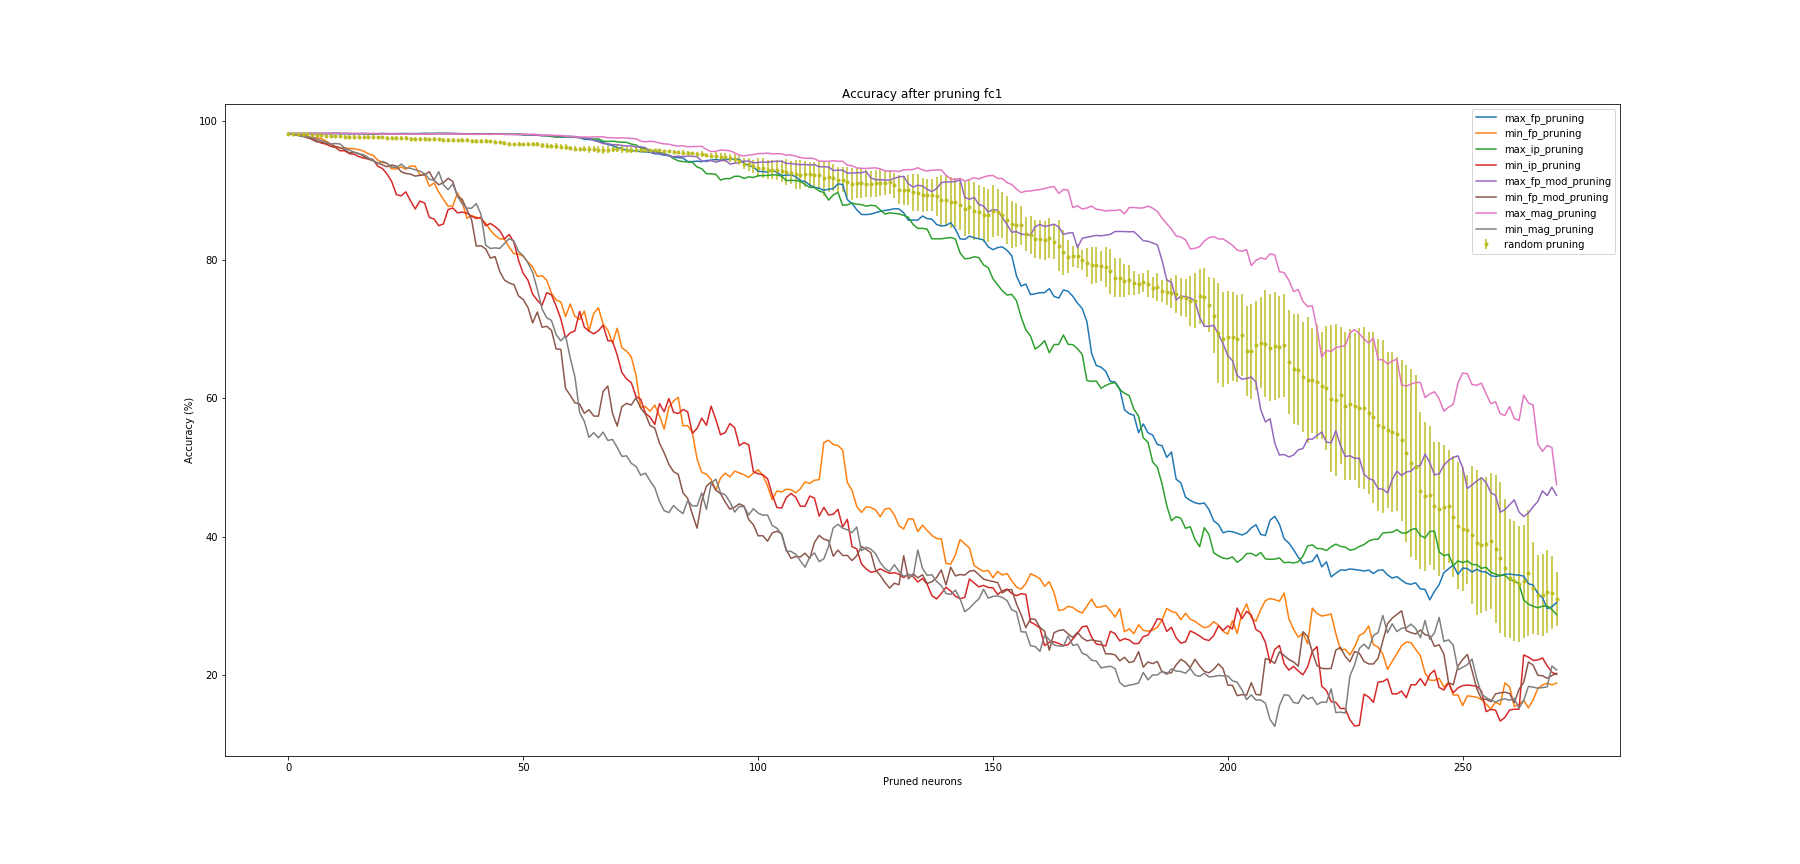
\includegraphics[width=1\linewidth]{{images/Lenet_fc1_pruned_acc}.png}
   \caption{Pruning the first fully connected layer of LeNet}
   \label{fig:lenet-fc1} 
\end{subfigure}

\begin{subfigure}[b]{\textwidth}
   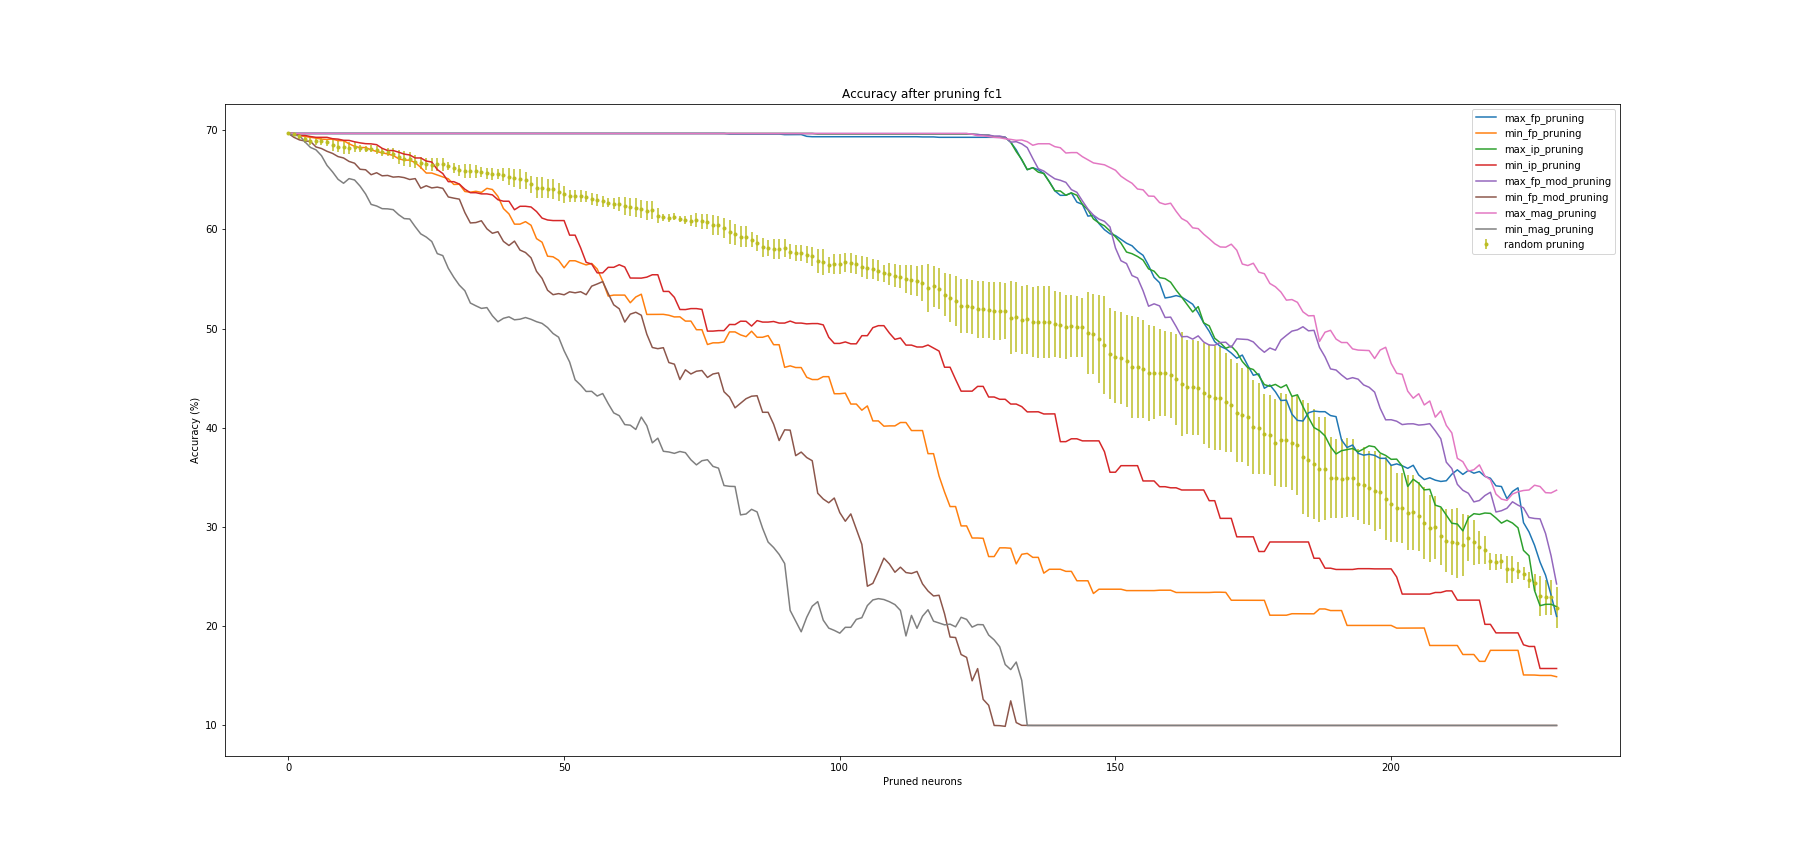
\includegraphics[width=1\linewidth]{{images/Conv2_fc1_combined_0.9_acc_13-10-2019_14:17:35}.png}
   \caption{Pruning the first fully connected layer of Conv-2}
   \label{fig:conv2-fc1}
\end{subfigure}
\caption{Comparison of different pruning metrics. \texttt{max\_mag\_pruning} (\texttt{min\_mag\_pruning}) corresponds to \textit{Magnitude pruning} that maximizes (minimizes) the Frobenius norm of the pruned matrix. \texttt{max\_fp\_pruning} (\texttt{min\_fp\_pruning}) corresponds to \textit{Frame-potential pruning}, it maximizes (minimizes) the frame-potential of the pruned matrix. For random pruning, averages were taken over 5 random experiments. Error bars were added with a width equal to the standard deviation, computed over the 5 random experiments, of the test accuracy obtained after pruning $i$ units.}
\end{figure}

\subsection{Visualizing training dynamics}

\subsubsection*{Method}
For a given weight matrix $\mathbf{W} \in \mathbb{R}^{m \times n}$, we would like to embed the norms of the rows of $\mathbf{W}$, $\|\mathbf{w}_1\|, \ldots, \|\mathbf{w}_m\|$, and the cosine similarities between the rows in a visualization. The cosine similarities can be obtained from the correlation matrix $\mathbf{X} = \hat{\mathbf{W}}\hat{\mathbf{W}}^T$, where $\hat{\mathbf{W}}$ is the matrix we get when normalizing the rows of $\textbf{W}$. A direct visualization of the weight vectors in an $n$-dimensional space is impractical, as $n$ can be very high (e. g. $n = 16384$ for the first fully connected layer of Conv-2). \\

Since we mainly care about magnitude and angle, the former being a feature of a weight vector, and the latter a property between weight vectors, an undirected weighted graph seems to be an appropriate choice of visualization. More specifically, we can construct a time-varying graph, with nodes representing individual weight vectors (single units), and weights between nodes (edges) representing the closeness between weight vectors as a function of the cosine similarity. Because edge weights must be positive and the entries of the correlation matrix $\mathbf{X}$ take values in $[-1, 1]$, we first transform the cosine similarity matrix to a cosine distance matrix, i. e. we compute $\mathbf{1} - \mathbf{X}$, whose entries lie in $[0, 2]$ (0 if colinear, 1 if orthogonal, 2 if opposed direction). Next we use a Gaussian function in order to turn these cosine distances into weights:

\begin{align*}
W(\textbf{w}_i, \textbf{w}_j) = \exp(-\frac{\text{dist}^2(\textbf{w}_i, \textbf{w}_j)}{\sigma^2}),
\end{align*}

where $\text{dist}^2(\textbf{w}_i, \textbf{w}_j) = (\mathbf{1} - \mathbf{X})_{ij}$ and $\sigma$ is a parameter which controls the width of the Gaussian. We have obtained an adjacency matrix which we can sparsify by removing the values below a certain threshold. \\

To summarize, we have a time-varying graph with nodes that can increase in size (corresponding to an increase in magnitude of the weight vector) and edge weights that can increase or decrease (reflecting a higher or smaller cosine similarity). The time-steps of the graph are training epochs, thus we observe how the weight vectors in a layer of a network evolve as the network gets trained. \\

To visualize the graph, we apply a Force Layout that models the nodes as charges and edges as links keeping them together. In addition to a repulsive charge force, a pseudo-gravity force keeps nodes centered in the visible area and avoids expulsion of disconnected subgraphs, while links are fixed-distance geometric constraints.


\subsubsection*{Observations}
Based on the self-regularization mechanism discussed in section \ref{section:prior} and the results of the pruning experiments in the previous section, some basic assumptions could be made on what the visualization would show. \cite{martin2018implicit} and \cite{nagarajan2019uniform} argue that after convergence, only a low-rank subspace of the space spanned by the rows of $\mathbf{W}$ is relevant to the output of the network. This low-complexity component is particularly receptive to training by SGD and dominates the output of the network, compared to the noisy component. This phenomenon would push weight vectors closer together and we would observe the emergence of edges with stronger weights. Moreover, using the results of \cite{brutzkus2019larger} and the fact that \textit{Frame-potential pruning} has proven to work better than random pruning, we would maybe expect to see the formation of clusters, but in particular outliers that don't fall into a cluster or aren't close to any other weight vector in the weight matrix. \\

The observations confirm our initial assumptions. In general, weight vectors move closer to each other, and often we see one big cluster, with some outliers that are not part of this big connected component (see fig. \ref{fig:conv2-fc1-final}). The emergence of the cluster probably indicates the presence of a low-rank subspace, that corresponds to the low-complexity component. Figure \ref{fig:conv2-fc1-final}, showing the graph we get for the first fully connected layer of Conv-2, is particularly interesting, because it highlights multiple phenomena discussed in section \ref{section:prior}. First, the aforementioned main big cluster, and the outliers around it, that in addition to not being part of the cluster are not close either to other weight vectors. Second, the emergence of removable units, which are units that do not experience a significant change during the training process and can be dropped out of the network without hurting the validation accuracy much. Note that in this case, since these removable units are not affected much by training, they are also not pushed towards the main cluster (most likely the low-rank subspace). This explains why in our pruning experiment for the same layer (fig. \ref{fig:conv2-fc1}), \textit{Magnitude pruning} and \textit{Frame-potential pruning} perform equally well, up to quite a high value of pruned units. In this particular example it becomes clear why magnitude is a good estimate of a unit's saliency. \\

A surprising result was that in some cases, even for larger networks, the weight vectors actually get clustered, as figure \ref{fig:vgg-conv16-final} shows. The threshold below which edges are removed was set to a value close to 1 for this graph. This means that if there is an edge between two nodes, the corresponding weight vectors almost overlap. The distinct clusters are clearly visible. The question was whether overlapping weight vectors would also produce similar outputs. Because bias-term, different magnitudes of the weight vectors and non-linearity of the activation function. has been added as a feature to the visualization. Reveal more repeated units. Indeed repeated units, corresponding to clustered weight vectors. \textbf{TODO: add viz result.} \\

The next section is motivated by the wish to examine more precisely the nature of the big cluster.

\begin{figure}[H]
\centering
\begin{subfigure}[b]{0.62\textwidth}
   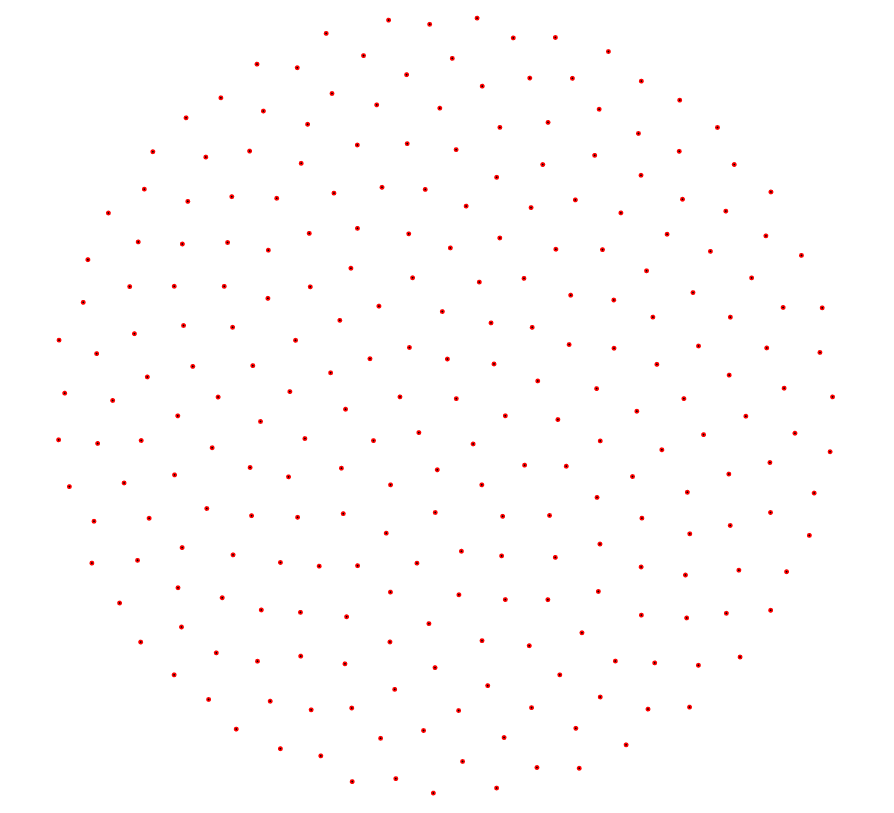
\includegraphics[width=\linewidth]{images/conv2-fc1-init.png}
   \caption{At initialization}
   \label{fig:conv2-fc1-init} 
\end{subfigure}

\begin{subfigure}[b]{0.62\textwidth}
   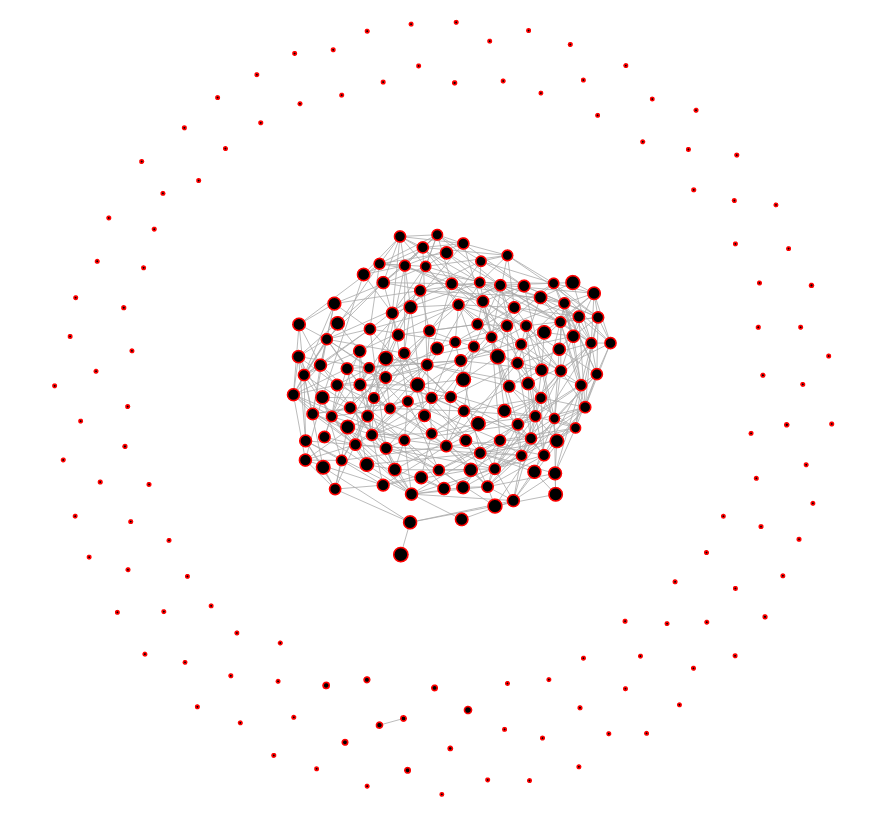
\includegraphics[width=\linewidth]{images/conv2-fc1-final.png}
   \caption{After convergence}
   \label{fig:conv2-fc1-final}
\end{subfigure}
\caption{Visualizing the training dynamics of the first fully connected layer of Conv-2}
\end{figure}

\begin{figure}[H]
\centering
	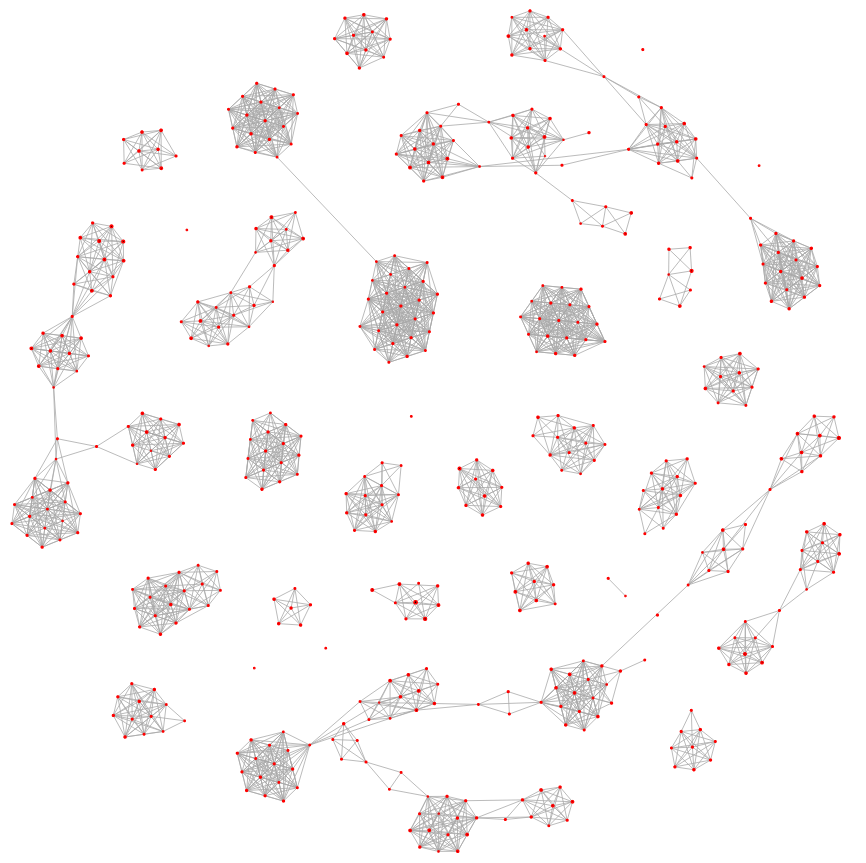
\includegraphics[scale=0.3]{images/vgg-conv16-final.png}
\caption{Cluster formation in the last convolutional layer of VGG19 during training}
\label{fig:vgg-conv16-final} 
\end{figure}

\subsubsection*{Additional observations}
TODO

\subsection{Subspace analysis}

In light of the findings of the previous sections and based on results in model compression that make use of matrix factorization ~\autocite{lebedev2014speeding} to compress deep neural networks, we propose a subspace analysis of chosen layer weight matrices, as a way to confirm the intuition we got from the visualization, and to learn more about the properties of models of different sizes. Inspired from the use of Random Matrix Theory of \cite{martin2018implicit} to study implicit self-regularization of neural networks, we analyze the Empirical Spectral Density (ESD) of layer correlation matrices. We also look at how performing a low-rank approximation of certain layer weight matrices affects the test accuracy, to see how informative the obtained low-complexity component is, depending on the model.

\subsubsection*{Random Matrix Theory}
For a given weight matrix $\mathbf{W} \in \mathbb{R}^{m \times n}$, the ESD of the correlation matrix $\mathbf{X} = \mathbf{W}\mathbf{W}^T, \mathbf{X} \in \mathbb{R}^{m \times m}$ is the density of eigenvalues $\rho(\lambda)$. If $\textbf{Z}$ denotes a $m \times n$ random matrix whose entries are independent identically distributed random variables with mean 0 and variance $\sigma^2 < \infty$, let

\begin{align*}
 \mathbf{Y}_n  = \frac{1}{n} \mathbf{Z} \mathbf{Z}^T, \mathbf{Y}_n \in \mathbb{R}^{m \times m}
\end{align*}

Then Marchenko-Pastur (MP) theory states that the ESD of $\mathbf{Y}_n$ has the limity density given by the MP distribution $\rho(\lambda)$. Note that $\rho(\lambda)$ is parametrized by the variance $\sigma^2$ and the aspect ratio $Q = n/m$ of the matrix $\mathbf{Z}$. In our case, $(\textbf{W})_{ij} \overset{\text{i.i.d.}}{\sim} \mathcal{N}(0, \sigma^2)$, where $\sigma^2$ is determined by the Gaussian Glorot distribution, and

\begin{align*}
 \mathbf{X} &= \mathbf{W}\mathbf{W}^T \\
 & = \frac{1}{n} (\sqrt{n}\mathbf{W})(\sqrt{n}\mathbf{W}^T)
\end{align*}

Since $(\sqrt{n}\mathbf{W})_{ij} \overset{\text{i.i.d.}}{\sim} \mathcal{N}(0, n\sigma^2)$, the limiting distribution of the ESD of $\mathbf{X}$ depends only on $Q = n/m$ and $n\sigma^2$.

\subsubsection*{Orthogonal Projections}
Let $\mathbf{A} \in \mathbb{R}^{m \times n}$ be a real (possibly rectangular) matrix with $m \geq n$. Suppose that $\mathbf{A} = \mathbf{U}\mathbf{\Sigma}\mathbf{V}^T$ is the Singular Value Decomposition (SVD) of $\mathbf{A}$. Recall that $\mathbf{U}$ and $\mathbf{V}$ are orthogonal matrices, and $\mathbf{\Sigma}$ is an $m \times n$ diagonal matrix with entries $(\sigma_1, \sigma_2, \dots, \sigma_n)$ such that $\sigma_1 \geq \sigma_2 \geq \dots \geq \sigma_n \geq 0$. Then the Eckart–Young–Mirsky theorem states that the best rank $k$ approximation to $\mathbf{A}$ in the spectral norm, denoted by $\|\cdot\|_2$, is given by

\begin{align*}
\mathbf{A}_k = \sum\limits_{i=1}^k \sigma_i \mathbf{u}_i \mathbf{v}_i^T,
\end{align*}

where $\mathbf{u}_i$ and $\mathbf{v}_i^T$ denote the $i^{\text{th}}$ column of $\mathbf{U}$ and $\mathbf{V}$ respectively. \\

We are interested in the row-space of a weight matrix $\mathbf{W} \in \mathbb{R}^{m \times n}$, to study how implicit self-regularization mechanism operate at the level of units. Thus we perform a rank $k$ approximation of the matrix $\mathbf{W}^T, k < m$, denoted by $\mathbf{W}_k^T$, before replacing $\mathbf{W}$ by $\mathbf{W}_k$ in the original network. To find a good value of $k$, the elbow method is applied to the function that maps the rank $k, 1 \leq k < m$, to the residuals obtained when performing a low-rank approximation of rank $k$.

\subsubsection*{Observations}

\begin{figure}[H]
\centering
	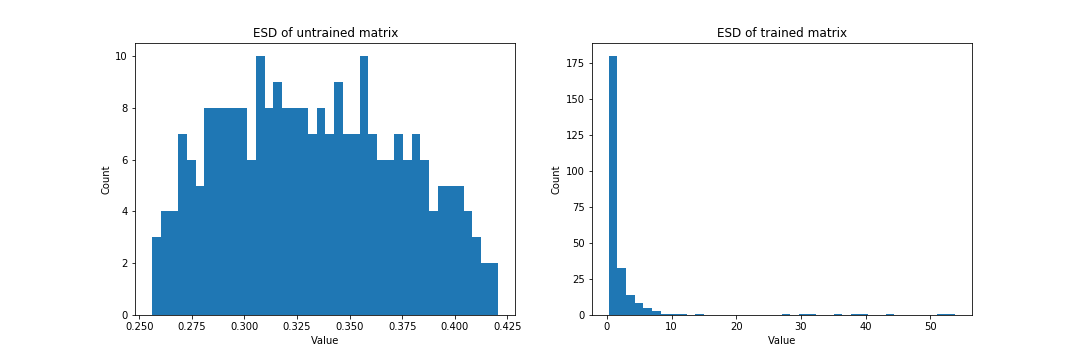
\includegraphics[scale=0.36]{images/conv2-fc1-svd-comp.png}
\caption{Empirical spectral densities of Conv-2 first fully connected layer correlation matrix, $Q = 64$.}
\label{fig:conv2-fc1-svd-comp} 
\end{figure}

\begin{figure}[H]
\centering
\begin{subfigure}[b]{\textwidth}
   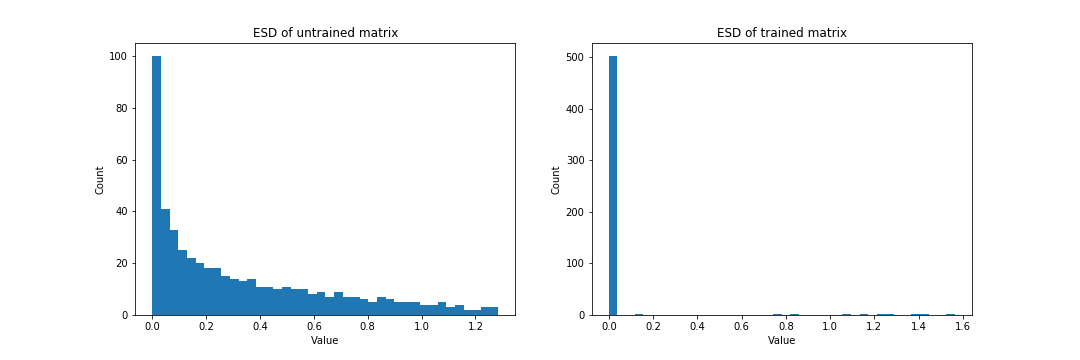
\includegraphics[width=1\linewidth]{images/vgg-fc1-svd-comp.png}
   \caption{First fully connected layer, $Q = 1$.}
   \label{fig:vgg-conv16-svd-comp}
\end{subfigure}

\begin{subfigure}[b]{\textwidth}
   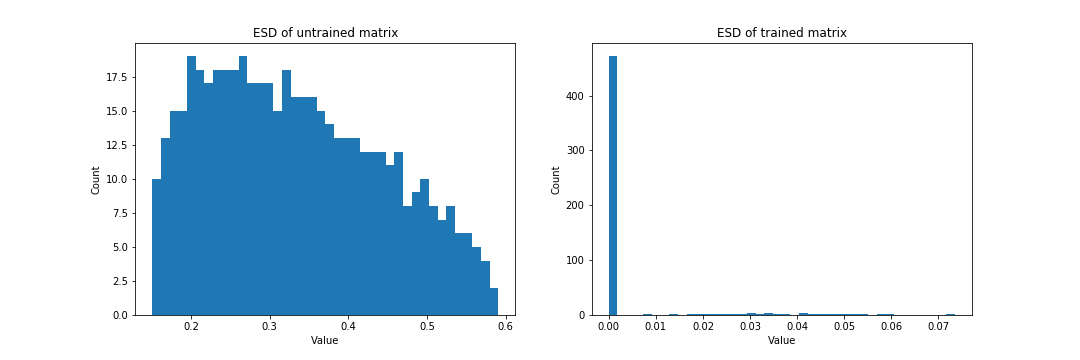
\includegraphics[width=1\linewidth]{images/vgg-conv16-svd-comp.png}
   \caption{Last convolutional layer, $Q = 9$.}
   \label{fig:vgg-conv16-svd-comp} 
\end{subfigure}
\caption{Empirical spectral densities of VGG19 layer correlation matrices}
\end{figure}

\begin{figure}[H]
\centering
\scalebox{0.9}
{\begin{tabular}{SSSS} \toprule
    {\textit{Network}} & {Conv-2} & {Conv-6} & {VGG19} \\ \midrule
    {\textit{Aspect ratio Q}} & {64} & {16} & {1} \\
    {\textit{Rank} $k$} & {10} & {10} & {10} \\
    {$100 \cdot \frac{ \| \mathbf{W}_k \|_F }{ \| \mathbf{W} \|_F }$}  & {71.61} & {61.43} & {99.99} \\
    {$a - a_{\text{proj}}$}  & {5.21} & {1.61} & {0} \\
    {\textit{Standard deviation}} & {\textbf{--}} & {\textbf{--}} & {\textbf{--}}\\ \bottomrule
\end{tabular}}
\caption{Low-rank approximation of first fully connected layer, tested with different architectures. For Conv-2 and Conv-6, values are averages taken over 10 random experiments. $a_{\text{proj}}$ denotes the accuracy obtained after replacing $\mathbf{W}$ by $\mathbf{W}_k$.}
\end{figure}

\section{Discussion}

Write conclusion and discuss future work. Even though emergence of removable and repeated units, implicit self-regularization operates at a different level. Subspace, study more in detail what they mean (singular vectors) in terms of the previous layer, to design better pruning methods.

\nocite{*}
\printbibliography

\end{document}
